\documentclass[12pt]{jarticle}
\usepackage[dvipdfmx]{graphicx}
\usepackage[dvipdfmx]{color}
\usepackage{here}
\title{原子核の変形と中性子ドリップラインに対するクーロン相互作用の効果}
\author{萩原健太}
\date{2023年1月21日}
\begin{document}

\begin{center}
    {\Large
        原子核の変形と中性子ドリップラインに対するクーロン相互作用の効果
    }
\end{center}
\vspace{1em}
\begin{flushright}
  201910867 萩原健太

  指導教員:中務孝
\end{flushright}


\section{背景}
複数個の陽子と中性子が集まった量子多体系である原子核を扱うエネルギー密度汎関数を用いることで、原子核の性質を系統的に調べることが出来る。
原子核の形に着目すると、陽子数や中性子数が魔法数に近い場合は球形に近く、魔法数から離れた場合には変形して存在することが実験と理論の両面から確認されている。
パリティ対称性と軸対称性を破らない変形が一般的であり、対称軸に対して細長く伸びたような変形をするプロレート型変形と、潰れたようなオブレート型変形の2種類に分けられる。
図\ref{fig:deformation}には一般的な変形を表示したが、上記の変形の他に対称性を破るような変形も予想されており、原子核の研究の大きなテーマの一つである。

\begin{figure}[H]
    \centering
    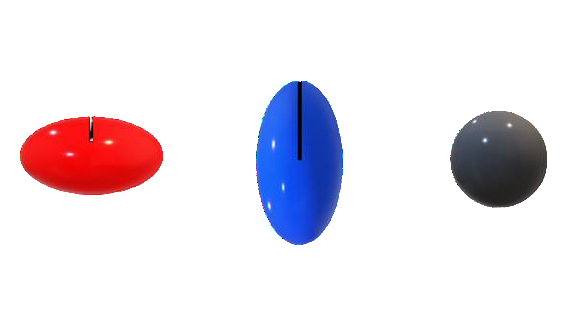
\includegraphics[width=100mm]{../変形図.png}
    \caption{原子核の一般的な変形}\label{fig:deformation}
\end{figure}

またそれぞれの元素における最大の中性子数についての研究も盛んに行われており、理論上存在可能な原子核はドリップラインと呼ばれている。
ドリップラインについての研究は宇宙での元素合成メカニズムなどにもつながり、学際的な関心も高い分野である。
本研究では化学ポテンシャルを$\lambda_n=\frac{dE}{dN}, \lambda_p=\frac{dE}{dZ}$のように設定し、これが負であることを束縛条件として中性子ドリップラインを定めた。

量子多体系である原子核の中では、正の電荷をもつ陽子を束縛させる強い相互作用とクーロン相互作用が支配的であるが、本研究ではクーロン相互作用に着目して計算・考察を行った。
過去の研究では斥力であるクーロン相互作用が、原子核の形状や中性子ドリップラインをはじめ様々な物理量にどのような影響を与えるのか報告されたことはなく、本研究は原子核の性質を知る上で重要な役割を果たすことが期待される。

\section{目的}
本研究の目的は、クーロン相互作用が原子核の変形度や中性子ドリップラインをはじめとする物理量に与える影響について、系統的な評価をすることである。

\section{方法}
本研究では原子核の変形と対相関を自己無頓着に決定することのできる計算プログラムであるHFBTHOを用い、陽子数$Z=2-120$の束縛する偶偶核を対象に数値計算を実行した。
束縛条件は陽子と中性子の化学ポテンシャルが負であることとして原子核の存在限界を決定した。


\section{結果}
陽子数$Z=2$から$Z=120$の偶偶核について計算を実行し、陽子、中性子の化学ポテンシャルがともに負の原子核の変形度$\beta$を 図\ref{fig:SLY4_ON}にプロットした。
変形度$\beta$は軸対象の変形を示しており、プロレート型の変形とオブレート型の変形の区別はせず、大きく変形している原子核を赤色で示している。
図\ref{fig:SLY4_OFF}にはクーロン相互作用を外した場合の計算結果をプロットした。
これらの結果よりクーロン相互作用の有無によって核図表全体に渡って変形度$\beta$が増加していること、および質量数の大きな領域では中性子ドリップラインが拡大していることが確認できる。
斥力のクーロン相互作用の効果で束縛される原子核が増加するというのは直感とは相反する結果である。
また中性子ドリップラインを拡大させている原子核に着目すると、変形核として存在することでドリップラインを拡大させている原子核と、球形核のままドリップラインを拡大させている原子核の2種類が存在することが確認できる。
これまでの研究で原子核が変形することによりエネルギー的に安定となることは指摘されているが、クーロン相互作用により球形のままエネルギー的により安定化するような原子核が存在することも大変興味深い。
球形のままドリップラインを拡大させている原子核は$Z=50,N=116-120$あたりに見られる。
\begin{figure}[ht]
    \centering
    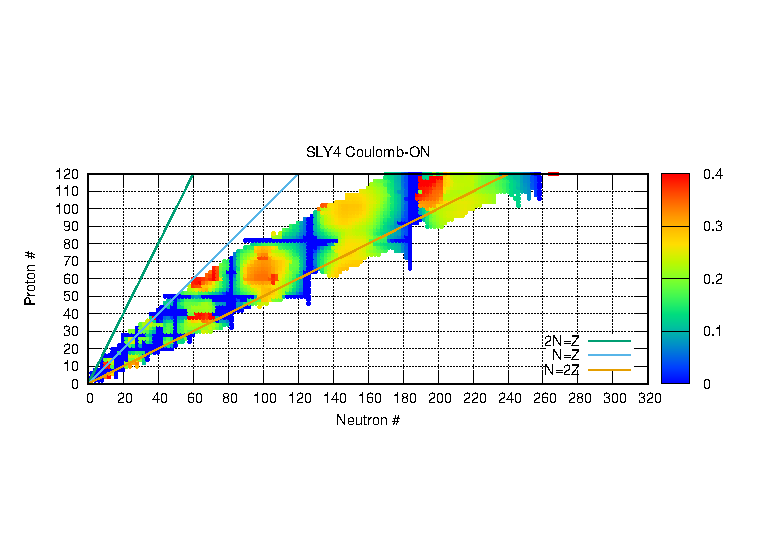
\includegraphics{../SLY4_ON.eps}
    \setlength\floatsep{0pt}
    \setlength\intextsep{0pt} 
    \setlength\textfloatsep{0pt}
    \caption{SLy4汎関数を用いた計算におけるクーロン相互作用を入れた場合の原子核の変形度$\beta$}\label{fig:SLY4_ON}
\end{figure}
\begin{figure}[H]
    \centering
    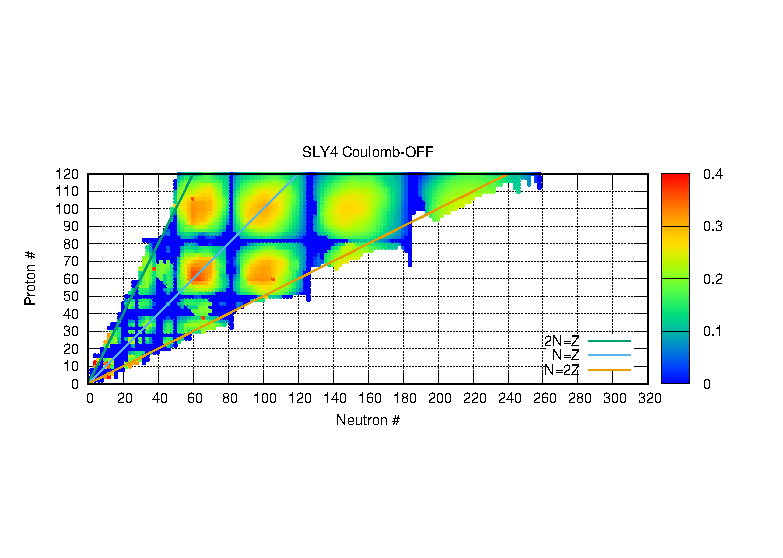
\includegraphics{../SLY4_OFF.eps}
    \setlength\floatsep{0pt}
    \caption{SLy4汎関数を用いた計算におけるクーロン相互作用を入れない場合の原子核の変形度$\beta$}\label{fig:SLY4_OFF}
\end{figure}

またクーロン相互作用と原子核の半径にも相関があることを確認した。
図\ref{fig:multi_SLY4_beta_radius_Z=50.eps}~図\ref{fig:multi_SLY4_beta_radius_Z=90.eps}では$Z=50$と$Z=90$の変形度$\beta$と半径を、中性子数の関数として表示した。
これらの図では核子の化学ポテンシャルは考慮せず、計算を実行したものを全てプロットした。
この結果からクーロン相互作用により変形の有無に依らずに原子核の半径が増加することが分かった。
これは斥力により陽子同士の間隔が広がり、それに呼応する形で原子核全体の半径が増加するようなメカニズムであると予想される。
また中性子のドリップライン内では有意な差として確認できるが、ドリップライン外側の中性子過剰核ではクーロン相互作用の有無に依る差が小さくなっていることも分かる。
これは陽子数に対して中性子の数が多くなることで、クーロン相互作用の効果が弱まることが要因であると考えられる。
\begin{figure}[H]
    \centering
    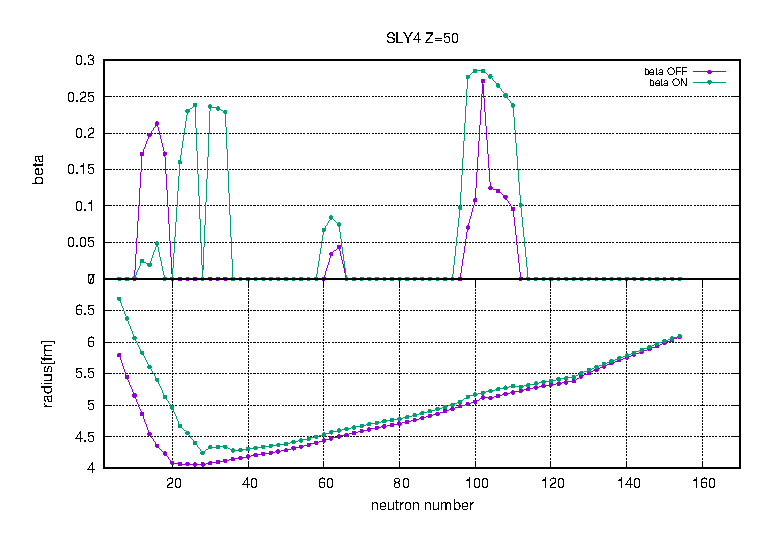
\includegraphics{../multi_SLY4_beta_radius_Z=50.eps}
    \setlength\floatsep{0pt}
    \caption{$Z=50$の変形度と半径}\label{fig:multi_SLY4_beta_radius_Z=50.eps}
\end{figure}
\begin{figure}[H]
    \centering
    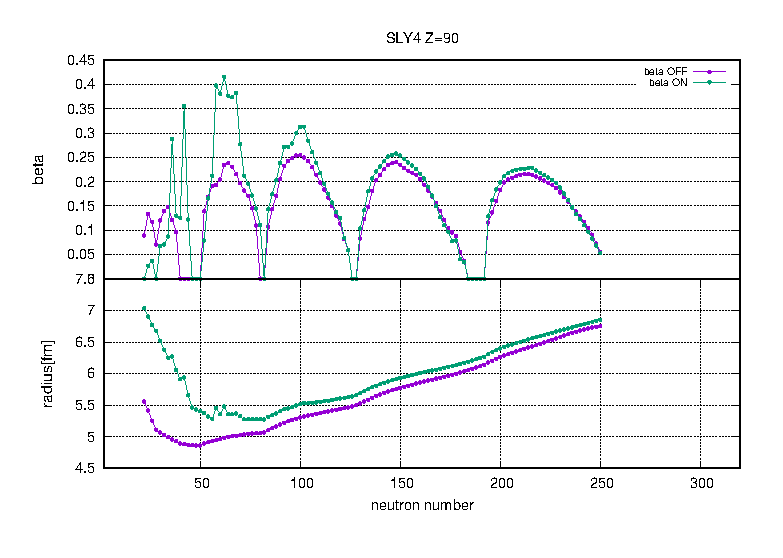
\includegraphics{../multi_SLY4_beta_radius_Z=90.eps}
    \setlength\floatsep{0pt}
    \caption{$Z=90$の変形度と半径}\label{fig:multi_SLY4_beta_radius_Z=90.eps}
\end{figure}



\subsection{中性子ドリップラインの拡大}
この項ではクーロン相互作用が原子核の半径を増加させることを出発点として、中性子ドリップラインが拡大するメカニズムに関する考察を進めていく。

まず半径が増加することで原子核の密度分布も変化することは自明である。
続いて一粒子のポテンシャルは密度分布とともに変化をしていくことも判明しており、それに従って1粒子のエネルギーが変化することで中性子ドリップラインが拡大すると考えた。
この予測を検証するため、球形のままドリップラインを拡大させている$Z=50,N=116$に着目して考察を行った。
図\ref{fig:SLY4_ON_Z=50_N=116_density}には、クーロン相互作用の有無により密度分布にどのような差が現れるか表示している。
\begin{figure}[H]
    \centering
    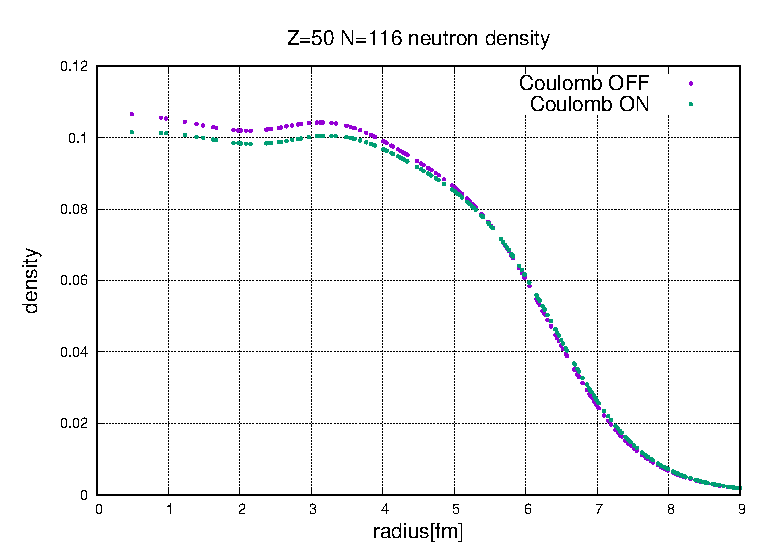
\includegraphics{../SLY4_Z=50_N=116_densityN.eps}
    \caption{$Z=50,N=116$の中性子密度分布}\label{fig:SLY4_ON_Z=50_N=116_density}
\end{figure}
図\ref{fig:SLY4_ON_Z=50_N=116_density}から分かるようにクーロン相互作用により中性子の密度分布は密度方向には潰れたような形になり、半径方向には広がる傾向が見られる。

%ログスケールやwith linesのプロットも試してみたのですが、あまり上手くいきませんでした。
%とりあえず点だけでプロットしてあります。
続いて$Z=50,N=116$内の中性子の1粒子エネルギーを図\ref{fig:SLY4_ON_Z=50_N=116_spe}に示す。
\begin{figure}[H]
    \centering
    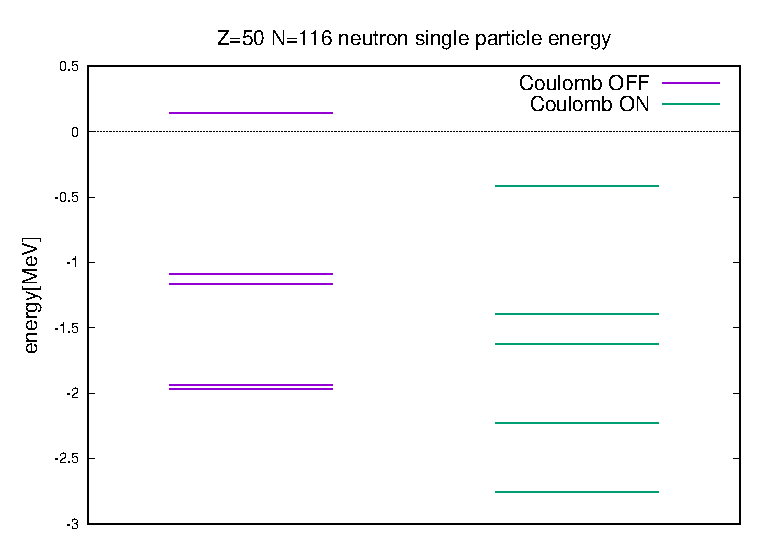
\includegraphics{../SLY4_Z=50_N=116_speN.eps}
    \caption{$Z=50,N=116$の中性子の一粒子準位}\label{fig:SLY4_ON_Z=50_N=116_spe}
\end{figure}
この図から明らかなようにクーロン相互作用によって中性子の1粒子エネルギーが減少することが確認できる。
さらに0エネルギー付近に注目すると、クーロン相互作用がない場合には$0[MeV]$を超えている準位が、クーロン相互作用がある場合には$0[MeV]$を下回っている。
これこそがクーロン相互作用が中性子ドリップラインを拡大しているメカニズムの一つである。

%球形核を例にとってクーロン相互作用が中性子ドリップラインを拡大させることを報告したが、次に変形核を詳細を調べることで、変形自体が中性子ドリップラインに与える影響について定量的に評価したい。

\section{考察}
\subsection{変形度}
この項ではクーロン相互作用によって基底状態の変形度がどのように変化するのかを確認する。
$Z=52,N=54$の原子核を例にとると、\ref{fig:SLY4_ON}および\ref{fig:SLY4_OFF}からクーロン相互作用によって変形度が増加していることがわかる。
図\ref{fig:Z=52_N=54_energy_beta}~図\ref{fig:Z=48_N=48_energy_beta}のようにエネルギーを変形度の関数としてプロットすることで、クーロン相互作用が変形度に与える影響について詳細に確かめた。
この際クーロン相互作用によるエネルギーのシフトは考慮しないよう、変形度が0となるエネルギーを揃えて比較した。
\begin{figure}[h]
    \centering
    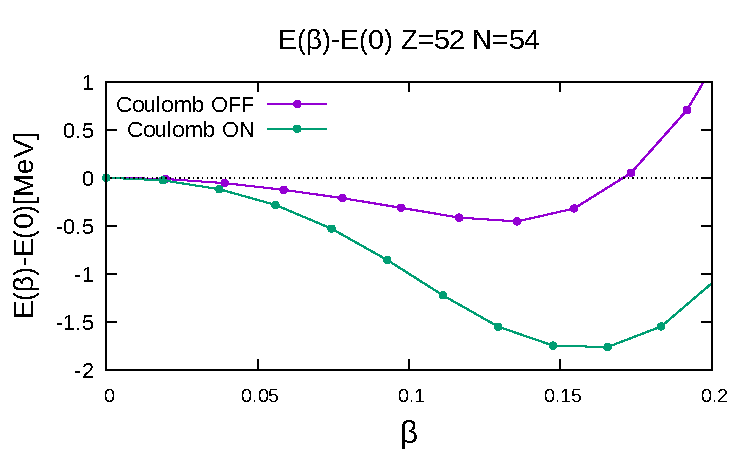
\includegraphics[width=120mm]{../Z=52_N=54_energy_beta.pdf}
    \caption{$Z=52,N=54$におけるエネルギーと変形度}\label{fig:Z=52_N=54_energy_beta}
\end{figure}
\begin{figure}[h]
    \centering
    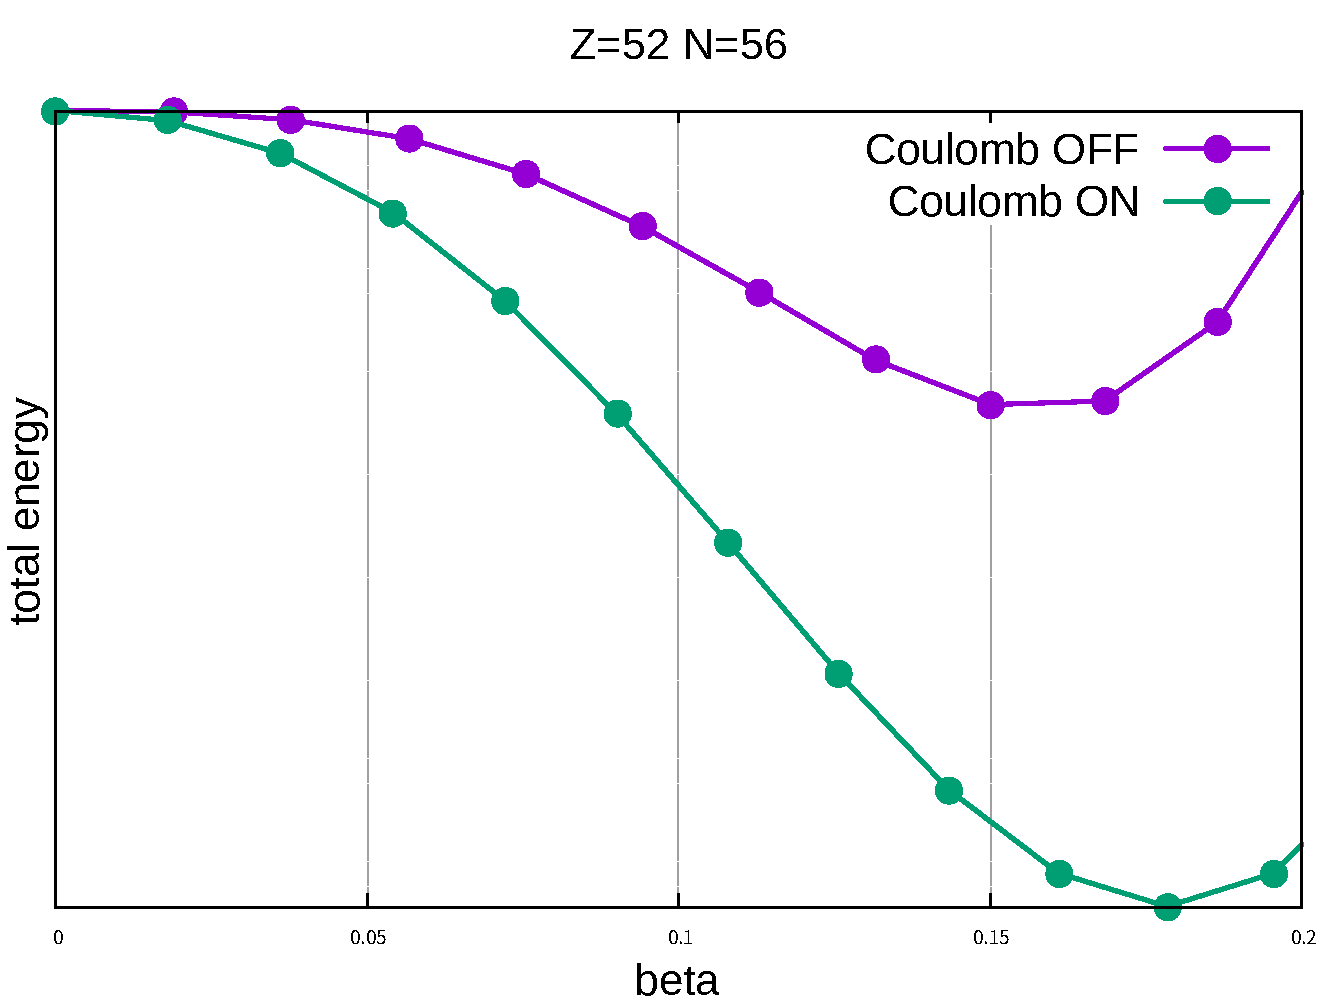
\includegraphics[width=120mm]{../Z=52_N=56_energy_beta.pdf}
    \caption{$Z=52,N=56$におけるエネルギーと変形度}\label{fig:Z=52_N=56_energy_beta}
\end{figure}
\begin{figure}[h]
    \centering
    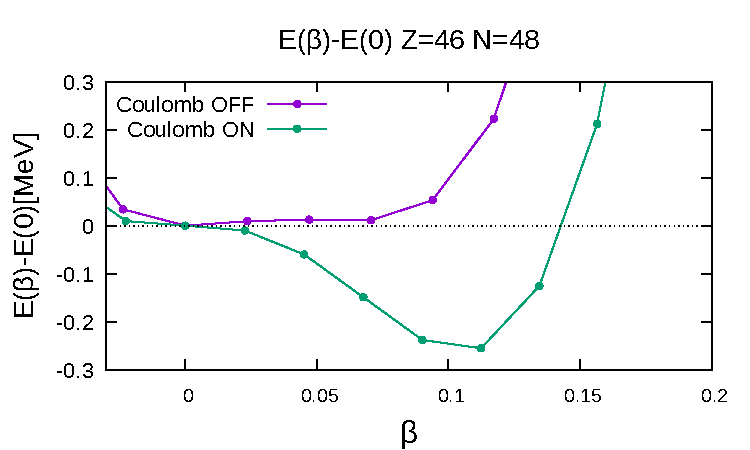
\includegraphics[width=120mm]{../Z=46_N=48_energy_beta.pdf}
    \caption{$Z=46,N=48$におけるエネルギーと変形度}\label{fig:Z=46_N=48_energy_beta}
\end{figure}
\begin{figure}[h]
    \centering
    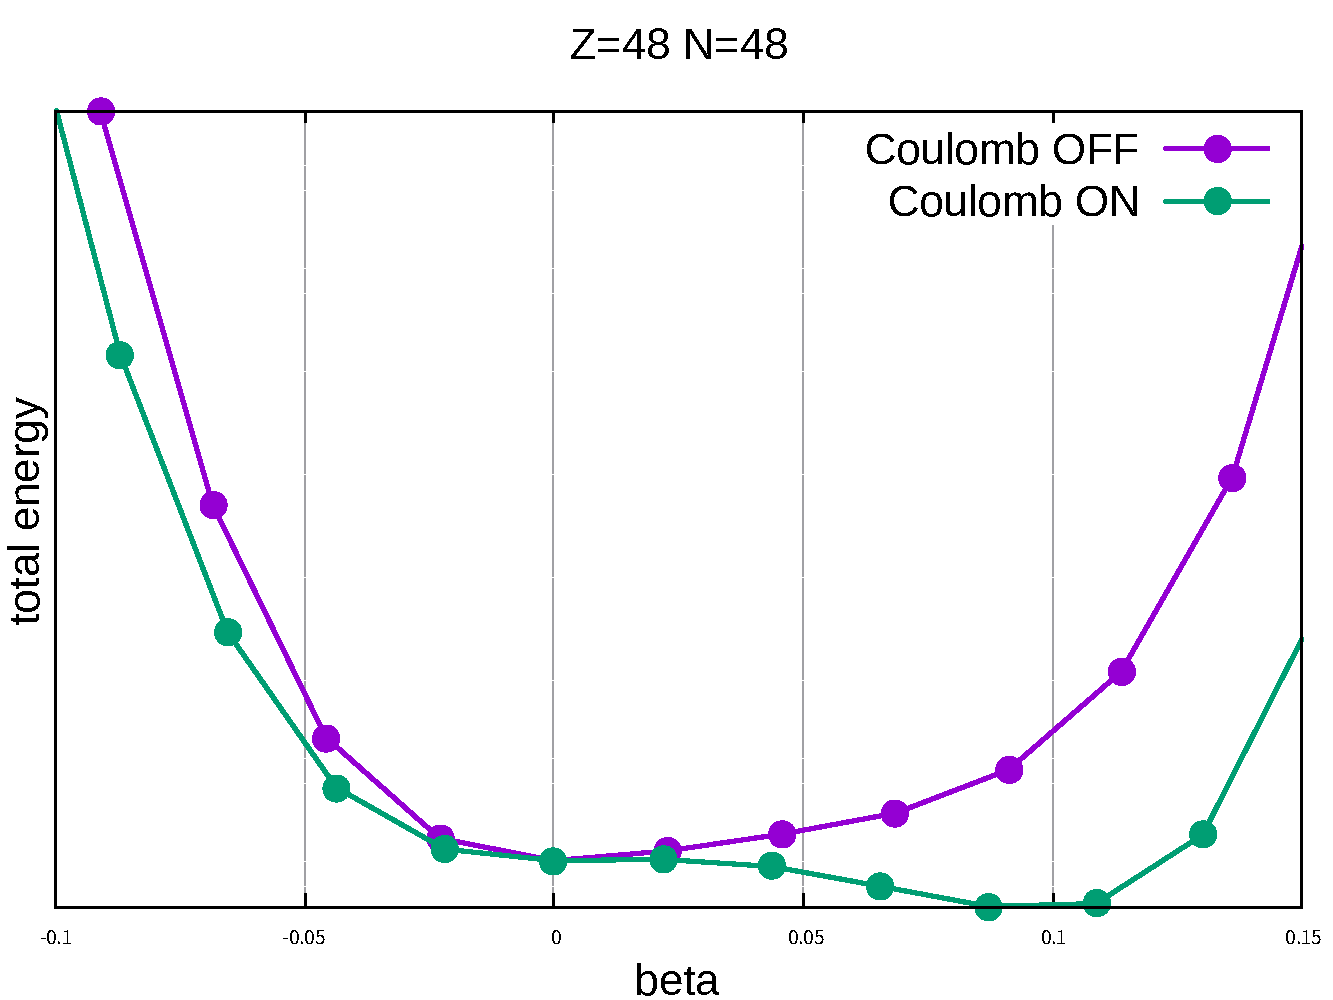
\includegraphics[width=120mm]{../Z=48_N=48_energy_beta.pdf}
    \caption{$Z=48,N=48$におけるエネルギーと変形度}\label{fig:Z=48_N=48_energy_beta}
\end{figure}
図\ref{fig:Z=52_N=54_energy_beta}~図\ref{fig:Z=48_N=48_energy_beta}に示した結果から、クーロン相互作用によって原子核はプロレート型の変形度を増加させる傾向にあることが確かめられる。
%オブレートはどうなるんだ?

\section{結論}
HFBTHOプログラムを用いた系統的な計算から、クーロン相互作用によって原子核の変形度は増加し、中性子ドリップラインは拡大することが分かった。
斥力により原子核の半径が増加することから核子の1粒子エネルギーが変化し、$0[MeV]$付近では一粒子準位が下がることが判明した。
その結果中性子の化学ポテンシャルが減少することで中性子ドリップラインが拡大することが分かった。
またエネルギーを変形度の関数として示すことで、クーロン相互作用が原子核の変形度を増加させることも示された。


\section{参考文献}
\begin{thebibliography}{99}
    \bibitem{Octupole_moment} Shuichiro Ebata and Takashi Nakatsukasa, Octupole deformation in the nuclear chart based on the 3D Skyrme Hartree-Fock plus BCS model, 2017
\end{thebibliography}
\end{document}